\documentclass[border=0.2cm]{standalone}
\usepackage[margin=1in]{geometry}
\usepackage{amsmath, amsthm, amssymb, graphicx, multicol, array}
\usepackage{tikz}
\usetikzlibrary{shapes, backgrounds}

\definecolor{blurple}{HTML}{CCCCFF}
\definecolor{mint}{HTML}{CCFFCC}
\definecolor{redder}{HTML}{FFCCCC}

\begin{document}
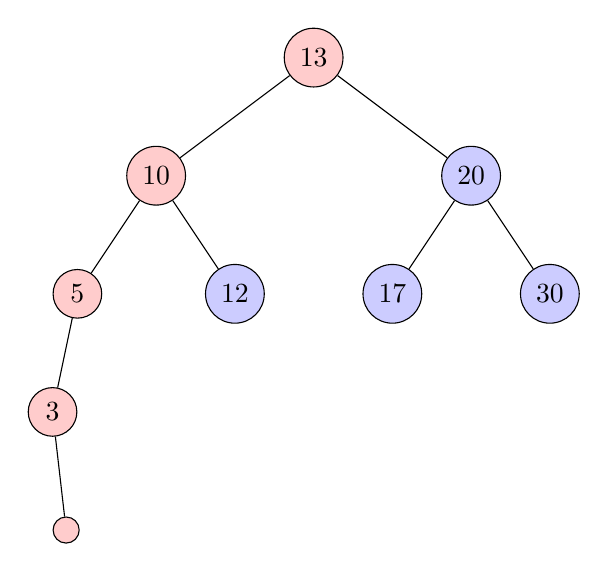
\begin{tikzpicture}[every node/.style={circle, fill=blurple, draw},level 1/.style={sibling distance=40mm},level 2/.style={sibling distance=20mm}, level 3/.style={sibling distance=10mm}]
  \node[fill=redder]{13}
  child {node[fill=redder] {10}
    child {node[fill=redder] {5}
      child {node[left, fill=redder] {3}
        child {node[right, fill=redder] {}}}}
    child {node {12}}}
  child {node {20}
    child{node {17}}
    child{node {30}}};
\end{tikzpicture}
\end{document}
